\documentclass[12pt]{article}

\usepackage{fontspec}
\usepackage{amsmath, amssymb, amsfonts}
\usepackage{graphicx}
\usepackage{hyperref}
\usepackage{color}
\usepackage{geometry}
\geometry{a4paper}

\usepackage{tikz}
\usetikzlibrary{calc, positioning}

\title{Mathématiques - révisions}
\date{Décembre 2023}

\begin{document}

	\maketitle

	\begin{enumerate}
		\item Résous les calculs vectoriels suivants :
		\begin{enumerate}
			\item $\left(2; 1; 0\right) + 3 \cdot \left(-2; 0; 1\right)$
			\item $\left(1; -1; 1\right) - \cdot \left(4; 1; 1\right)$
			\item $\left(1; -1; 1\right) + \vec{0}$
		\end{enumerate}
	
		\item Additionne graphiquement $\vec{u}$ et $\vec{v}$ :
			\begin{center}
				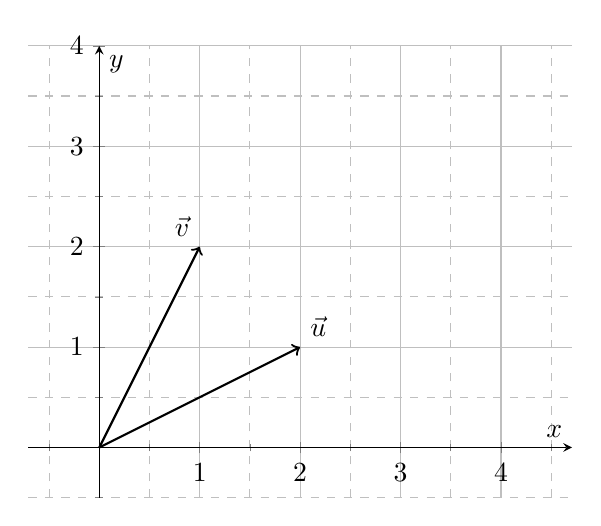
\begin{tikzpicture}
					\begin{axis}[
						width=.7\linewidth,
						axis lines=center,
						xlabel={$x$},
						ylabel={$y$},
						xmin=0, xmax=4,
						ymin=-0.5, ymax=4,
						axis equal,
						grid=both,
						minor tick num=1,
						minor grid style={dashed}
						]
						
						\addplot[->, thick] coordinates {(0, 0) (2, 1)} node[above right] {$\vec{u}$};
						\addplot[->, thick] coordinates {(0, 0) (1, 2)} node[above left] {$\vec{v}$};
					\end{axis}
				\end{tikzpicture}
			\end{center}
			\vspace{8em}
		
		\item Calcule graphiquement $\vec{u} - \vec{v}$ :
			\begin{center}
				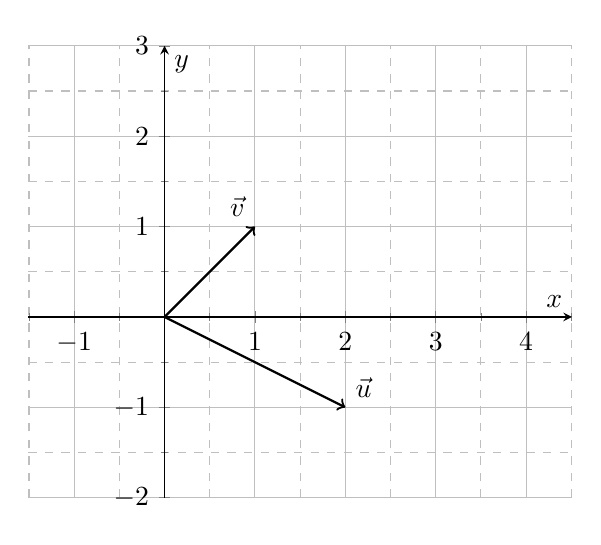
\begin{tikzpicture}
					\begin{axis}[
						width=.7\linewidth,
						axis lines=center,
						xlabel={$x$},
						ylabel={$y$},
						xmin=0, xmax=3,
						ymin=-2, ymax=3,
						axis equal,
						grid=both,
						minor tick num=1,
						minor grid style={dashed}
						]
						
						\addplot[->, thick] coordinates {(0, 0) (2, -1)} node[above right] {$\vec{u}$};
						\addplot[->, thick] coordinates {(0, 0) (1, 1)} node[above left] {$\vec{v}$};
					\end{axis}
				\end{tikzpicture}
			\end{center}
	
		\item Les vecteurs suivants sont-ils colinéaires ? Orthogonaux ? Aucun des deux ?
			\begin{enumerate}
				\item $\left(1; 0; 1\right)$ et $\left(-3; 0; 3\right)$
				\item $\left(1; -1; 0\right)$ et $\left(0; 0; 1\right)$
				\item $\left(2; 1; 0\right)$ et $\vec{0}$
				\item $\left(1; 2; 3\right)$ et $\left(-1; -2; -3\right)$
				\item $\left(2; -1; 3\right)$ et $\left(-3; 0; 2\right)$
				\item $\left(1; -1; 3\right)$ et $\left(\frac{-5}{2}; \frac{5}{2}; \frac{-15}{2}\right)$
			\end{enumerate}
		
		\item Soit les vecteurs $\vec{u} = \left(3; 1; 1\right)$ et $\vec{v} = \left(1; 2; -5\right)$.
			\begin{enumerate}
				\item $\vec{u}$ et $\vec{v}$ sont-ils orthogonaux ?
				\item Soit $\vec{w} = \left(1; a; b\right)$. Détermine $a$ et $b$ pour que $\vec{w}$ soit orthogonal à $\vec{u}$ et $\vec{v}$.
			\end{enumerate}
		
		\item On donne les points $A \equiv \left(1; 2; -1\right), B \equiv \left(-3; m; 1\right), C \equiv \left(2; -1; 2\right)$ et $D \equiv \left(0; 2; 3\right)$. Quelle valeur faut-il donner à $m$ pour que :
			\begin{enumerate}
				\item les vecteurs $\vec{AB}$ et $\vec{CD}$ soient colinéaires ?
				\item les vecteurs $\vec{AB}$ et $\vec{CD}$ soient orthogonaux ?
			\end{enumerate}
		
		\item Une poutre repose sur le sol et à l'angle des murs d'un local. Utilise les données de la figure ci-dessous pour déterminer la longueur de la poutre :
		\vspace{2em}
			\begin{center}
				\begin{tikzpicture}
					\begin{axis}[
						view={105}{30}, 
						axis lines=center,
						xlabel={$x$},
						ylabel={$y$},
						zlabel={$z$},
						xtick={0,1,...,4},
						ymax=3, ymin=0,
						ztick={0,1,...,4},
						grid=major,
						]
						
						\addplot3[red, thick] coordinates {(0, 0, 3) (3, 2, 0)};
						\addplot3[dashed] coordinates {(3, 2, 0) (3, 0, 0)};
						\addplot3[dashed] coordinates {(3, 2, 0) (0, 2, 0)};
						
					\end{axis}
				\end{tikzpicture}
			\end{center}
			
		\item Donne l'équation vectorielles des figures suivantes :
			\begin{enumerate}
				\item La droite $D$ de vecteur directeur $\left(1; -2; 3 \right)$ et passant par le point $\left(1; 0; 1\right)$.
				\item Le plan $P$ de vecteurs directeurs $\left(1; 1; 3\right)$ et $\left(-2; 1; 1\right)$ et passant par le point $\left(0; 1; 0\right)$.
			\end{enumerate}
		
		\item Soit le plan $P$ d'équation $P \equiv \vec{x} = k_1 \cdot \left(0; 1; 2\right) + k_2 \cdot\left(3; 2; -1\right) + \left(1; 1; 1\right), ~(k_1, k_2 \in \mathbb{R})$. Donne l'équation d'un plan $R$ \textbf{orthogonal} à $P$.
		
		\item Donne l'équation paramétrique de la droite qui passe par les points $A$ et $B$ représentés dans le repère orthonormé ci-dessous :
			\begin{center}
				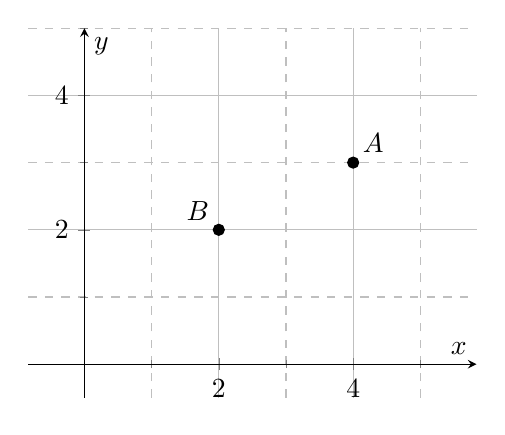
\begin{tikzpicture}
					\begin{axis}[
						width=.6\linewidth,
						axis lines=center,
						xlabel={$x$},
						ylabel={$y$},
						xmin=0, xmax=5,
						ymin=-0.5, ymax=5,
						axis equal,
						grid=both,
						minor tick num=1,
						minor grid style={dashed}
						]
						
						\addplot[only marks, mark=*] coordinates {(4, 3)} node[above right] {$A$};
						\addplot[only marks, mark=*] coordinates {(2, 2)} node[above left] {$B$};
						
					\end{axis}
				\end{tikzpicture}
			\end{center}
		
		\vspace{3em}
		
		\item Soit les figures suivantes :
			\begin{itemize}
				\item Le plan $P$ d'équation $P \equiv \vec{x} = k_1 \cdot \left(1; 1; 1\right) + k_2 \cdot\left(0; 1; 2\right) + \left(0; 0; 1\right), ~(k_1, k_2 \in \mathbb{R})$.
				\item La droite $D$ d'équation $D \equiv \vec{x} = k \cdot \left(1; -2; a\right) + \left(3; 2; 1\right), ~(k \in \mathbb{R})$.
			\end{itemize}
			Pour quelle valeur du paramètre $a$ la droite $D$ sera-t-elle orthogonale au plan $P$ ?
			
		\item Soit le plan $P$ défini par les points $A \equiv \left(1; 1; -1\right)$, $B \equiv \left(2; 2; 0\right)$ et $C \equiv \left(2; 5; 2\right)$. Donne les équations paramétrique et cartésienne de $P$.
		
		\item On donne le plan $P \equiv 3x + 2y - 5z = -4$. Détermine les points $A$, $B$ et $C$ de ce plan si :
			\begin{enumerate}
				\item $A$ d'abscisse 3 et d'ordonnée 1
				\item $B$ d'abscisse -1 et d'ordonnée 4
				\item $C$ d'abscisse 2 et d'ordonnée 2
			\end{enumerate}
		
		\item Vrai ou faux ? Justifie:
			\begin{enumerate}
				\item Tout multiple d'un vecteur directeur d'une droite est un vecteur directeur de cette droite.
				\item Le système $\begin{cases}
					2x - 4y + 3z - 1 = 0\\
					3x - 6y + 4,5z +7 = 0
				\end{cases}$ est un système d'équations cartésiennes d'une droite.
				\item Deux droites sont parallèles si elles ont un même vecteur directeur.
				\item Deux plans sont parallèles si un vecteur directeur de l'un est un vecteur directeur de l'autre.
				\item Deux plans sont orthogonaux si un vecteur normalà l'un est orthogonal à un vecteur normal à l'autre.
				\item Deux plans sont parallèles s'ils ont un même vecteur normal.
			\end{enumerate}
	
	\end{enumerate}
	
\end{document}